\section{Introduction}\label{sec:introduction}

Blockchains exploit the redundant, concurrent execution of the same
transactions on a decentralized network of many machines,
in order to enforce their execution in accordance with
a set of predefined rules. Namely, blockchains make it hard, for a single machine,
to disrupt the semantics of the transactions or their ordering: a misbehaving single machine
gets immediately put out of consensus and isolated. Bitcoin~\cite{Nakamoto08,book-mastering-bitcoin}
has been the first blockchain's success story. Here
transactions are programmed in a non-Turing complete bytecode language,
almost exclusively used to implement transfers of units of coins between \emph{accounts}.

A few years after Bitcoin, another blockchain, called
Ethereum~\cite{Buterin13,AntonopoulosW18}, introduced the possibility of programming
transactions in an actual, imperative and Turing-complete programming language, called Solidity.
Solidity's code is organized in \emph{smart contracts}, that can be seen as
objects that control money. A smart contract is essentially an agreement between two or more parties that can be automatically enforced without the need for a trustworthy intermediary~\cite{ebp}.
Ethereum's transactions can hence execute much more than coin transfers. Namely,
they run object constructors and methods, which results in a sort
of \emph{world computer} that persists the same objects inside the memory of all the
computers composing the blockchain's network.

In Solidity's bytecode,
non-primitive values are referenced through a very general
\<address> type. For instance, a Solidity method
\<child(Person p, uint256 n) returns Person> actually compiles
into \<child(address p, uint256 n) returns address>, losing most
type information~\cite{CrafaPZ19}.
Since, at run time, it is the bytecode that gets executed,
everything can be passed for \<p>, not just a \<Person> instance, as illustrated in Fig.\,\ref{figure.solidity_problem}.
The compiler cannot even enforce strong typing
by generating defensive type instance checks and casts, because
values are unboxed in Ethereum: they have no attached
type information at run time,
they are just numerical \emph{addresses}.
It follows that inside the \<child> method, an eventual call to a \<Person>'s method
on \<p> might actually execute any arbitrary code, if \<p> is not a \<Person>.
In other words, Solidity is not strongly typed.
Consequently, it is highly discouraged, in Solidity, to call methods on parameters passed
to another method, such as on \<p> passed to \<child>, since an attacker can pass crafted
objects for \<p>, with arbitrary implementations for their methods,
which can result in the unexpected execution of
dangerous code. This actually happened in the case of the infamous DAO hack~\cite{dao16}, that
costed millions of dollars.

\begin{figure}[ht]
\centering
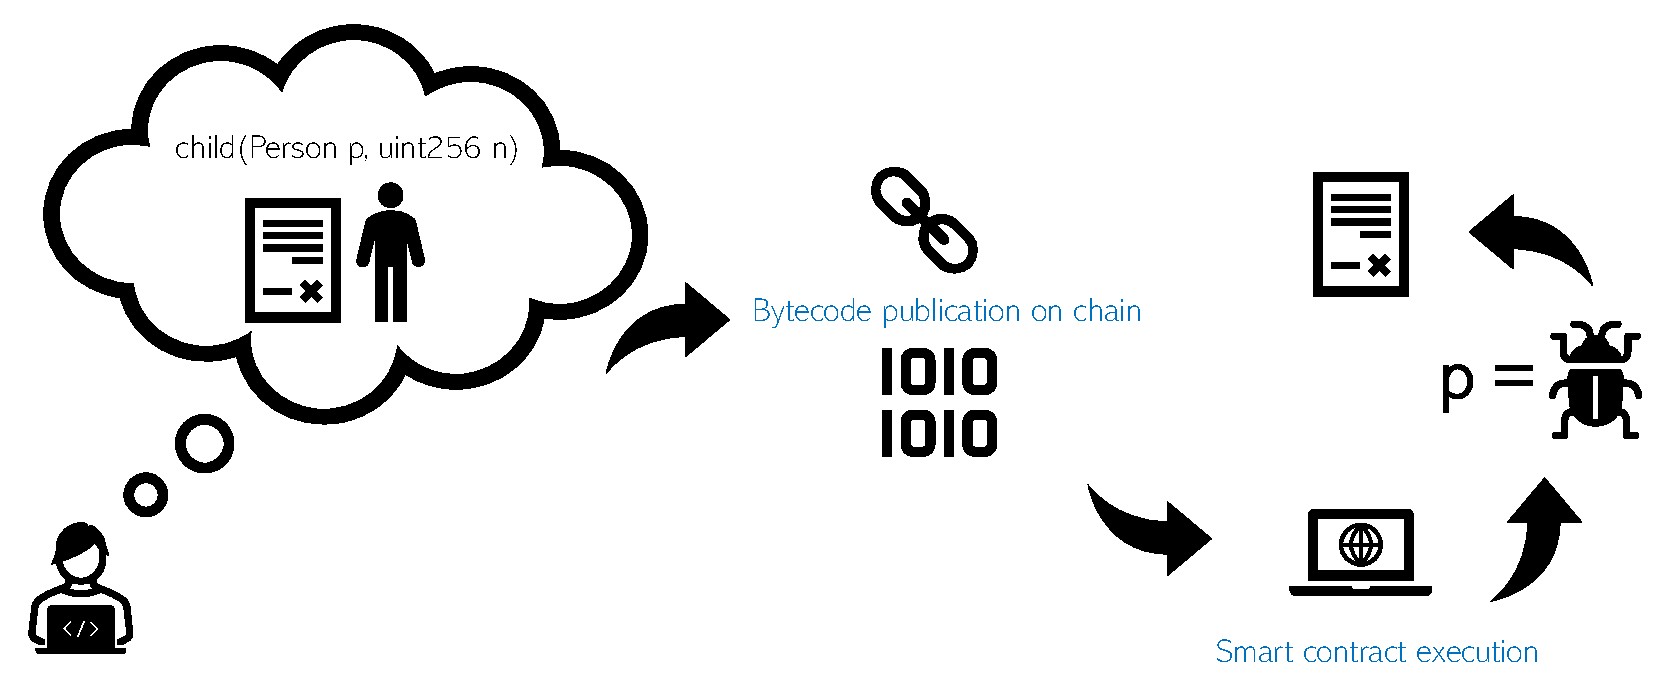
\includegraphics[width=.9\linewidth]{figures/solidity_problem}
\caption{Example of possible problem that can occur in Solidity due to the absence of a strong typing mechanism.}
\label{figure.solidity_problem}
\end{figure}

Strong typing is one of the reasons that push towards the adoption
of \emph{traditional} programming languages for smart contracts. For instance,
the Cosmos blockchain~\cite{cosmos} uses Go. The
Hotmoka blockchain~\cite{hotmoka} uses a subset of Java
for smart contracts, called Takamaka~\cite{Spoto19,Spoto20}.
Hyperledger~\cite{hyperldeger} allows Go and Java.
Another reason is the availability of modern
language features, that are missing in Solidity,
such as \emph{generics}\ie the possibility of using
type variables. Generics are a powerful and very useful facility for programming
smart contracts, since they allow one to personalize the behaviour of such contracts and partially overcome their inherent incompleteness~\cite{ebp}. In Java source code, generics are strongly typed, if no \emph{unchecked operations}
are used~\cite{NaftalinW06}, as it will always be the case in this paper.
However, generics might have security issues
at the level of compiled Java code and this paper originated from a
real issue that we found in our code.




The contribution of this paper is to show a real-life
use of generics for an actual smart contract contained in the support
library of the Takamaka language, and to demonstrate that a na\"{i}ve use
of Java generics can lead to a code security vulnerability that
allows an attacker to earn money by exploiting someone else's work, with both economical and legal side effects.
This paper will provide a fix to that specific issue,
by proposing a re-engineering of the code that forces the compiler to generate defensive checks.
More generally, this paper can be useful for the definition of
bytecode languages for future smart contract languages, by
learning from the weaknesses of Java bytecode.

The remainder of this paper is organized as follows.
Sec.~\ref{sec:java_generics} discusses the management of generics in Java.
Sec.~\ref{sec:takamaka} presents the basic notions about the Takamaka language for smart contracts in Java.
Sec.~\ref{sec:shared_entities} shows our real-life Java smart
contracts for shared entities, that use generic types.
Sec.~\ref{sec:validators} shows the instantiation of the shared entities to implement the validators' set
of a proof of stake blockchain.
Sec.~\ref{sec:attack} shows that a na\"{i}ve
deployment of a subclass of the validators' set leads to a code vulnerability.
Sec.~\ref{sec:fix} presents a fix to that vulnerability.
Sec.~\ref{sec:related_work} discusses some related work.
Sec.~\ref{sec:conclusion} concludes.

This paper is a revised and extended version of~\cite{BeniniGMS21}.
In comparison to that paper, Sec.~\ref{sec:takamaka} and
Sec.~\ref{sec:validators} are new; eight figures have been added;
all other sections have been expanded.
